\documentclass[titlepage]{article}
\usepackage[left=15mm,right=15mm,top=1in,bottom=1in]{geometry}
\usepackage{framed}
\usepackage{caption}
\usepackage{amsmath}
\usepackage{imakeidx}
\usepackage{graphicx}
\usepackage{array}
\usepackage{tikz}
\usetikzlibrary{automata,positioning,decorations.pathmorphing,shapes}

\newcolumntype{C}[1]{>{\centering\arraybackslash} m{#1cm}}
\graphicspath{{./img/}}

\makeindex

\title{Autonomous Pool Playing Robot\\~\\\textbf{\Huge{Hazard Analysis}}}
\author{
	Ernest Selman\\selmae@mcmaster.ca\\1201291\\~\\\and
	Guy Meyer\\meyerg@mcmaster.ca\\1320231\\~\\\and
	Eric Le Fort\\leforte@mcmaster.ca\\1308609\\~\\\and
	Andrew Danha\\danhaas@mcmaster.ca\\1223881\\~\\\and
	Derek Savery\\saverydj@mcmaster.ca\\1219142\\~\\\and
	Max Moore\\moorem8@mcmaster.ca\\1320009
}
\begin{document}
\maketitle
\tableofcontents
\listoftables
\listoffigures


\vfill
\begin{table}[!htbp]
\centering
\begin{tabular}{| C{3} | C{2} | C{5} | C{2.5} |}\hline
	Date			&Revision \#	&Comments						&Authors\\\hline
	05/01/2017		&0				&- Initial document creation	&Eric Le Fort\\\hline
	06/01/2017		&0				&- First draft				&Eric Le Fort\\\hline
	11/03/2017		&1				&- Revision 1				&Andrew Danha Derek Savery\\\hline
\end{tabular}
\caption{Revision History}
\end{table}
\newpage
\section{Overview}
This document's purpose is to help illustrate potential hazards associated with the automated pool-playing robot and how those hazards are to be addressed. Hazards include both safety risks to users as well as structural/monetary risks to the machine. The Hazards section will describe the section in more detail as well as provide an overall Fault-Tree Analysis (FTA) for this system. Each hazard will have its own subsection which will describe the hazard, discuss mitigation and/or plans of avoidance as well as provide a more detailed view of the portion of the FTA it concerns.\\~\\
Certain sections may refer to the supporting documents: \textit{High-Level Hardware Design} and \textit{High-Level Software Design} for this project.

\subsection{Naming Conventions \& Definitions}
This section outlines the various definitions, acronyms and abbreviations that will be used throughout this document in order to familiarize the reader prior to reading.
\subsubsection{Definitions}
Table \ref{tab:Definitions} lists the definitions used in this document. The definitions given below are specific to this document and may not be identical to definitions of these terms in common use. The purpose of this section is to assist the user in understanding the requirements for the system.
\begin{table}[h!]
\centering
\caption{Definitions}
\begin{tabular}{| C{6} | p{6cm} |}\hline
	\textbf{Term}	&\textbf{\centering Meaning}\\\hline
	X-axis					&Distance along the length of the pool table\\\hline
	Y-axis					&Distance across the width of the pool table\\\hline
	Z-axis					&Height above the pool table\\\hline
	End-effector			&The end of the arm that will strike the cue ball\\\hline
	$\theta$				&Rotational angle of end-effector\\\hline
	Cue 					&End-effector\\\hline
\end{tabular}
\label{tab:Definitions}
\end{table}

\subsubsection{Acronyms \& Abbreviations}
Table \ref{tab:Acronyms} lists the acronyms and abbreviations used in this document.
\begin{table}[h!]
\centering
\caption{Acronyms and Abbreviations}
\begin{tabular}{| p{6cm} | p{6cm} |}\hline
	\textbf{Acronym/Abbreviation}	&\textbf{Meaning}\\\hline
	VR								&Visual Recognition\\\hline
	$\mu$C							&Micro-Controller\\\hline
	FTA								&Fault-Tree Analysis\\\hline
\end{tabular}
\label{tab:Acronyms}
\end{table}

\newpage
\section{Background}
The potential hazards associated with this system can be found by examining other products and their solutions to the respective hazards.\\~\\
This machine uses a similar traversal system as a household 3D printer. 3D printers contain multiple moving parts and are labeled with warnings to keep hands and fingers clear during operation, due to the multiple pinch points. Some 3D printers solve this issue by enclosing the entire printer in a sealed environment. 3D printers can also pose as an electrical shock hazard, as with any electrical equipment. 3D printers also include delicate electronics and sensors. Users are advised to handle with care since hampering with them can cause the 3D printer to operate incorrectly.\\~\\

\section{Scope and Boundary}
Hazard analysis performed in this document will be contained to the scope of mechanical, electrical, and software aspects of the machine.\\~\\
Integrity of the pool table, pool balls, and pool cues will not be discussed. Robustness of raw materials used in the physical build of the mechanical system will not be discussed. Reliability of the motors, sensors, transformer unit, AC/DC unit, electrical wiring, motor controllers, $\mu$C, and pc unit will not be discussed unless it relates to a specific way in which the components are to be used. The stated individual components will in this way be treated as black-box systems in which the reliability of outputs are assumed.\\~\\
All hazards are applicable to the case in which a single user is interacting with the machine with the assumption made that the user is not behaving in an intentionally destructive manner.

\newpage
\section{Hazards}
This section will outline all identified hazards associated with this system. Each hazard will be described, plans for avoiding and/or mitigating the effects of that risk will be stated, and a more-detailed FTA for that hazard will be provided.\\~\\
The following diagram is the FTA for the system with the hazard specific details abstracted out.\\
\begin{center}
	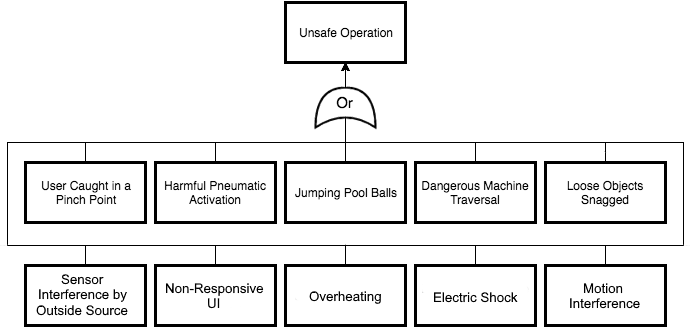
\includegraphics[width=0.9\textwidth]{SystemFTA.png}
\captionof{figure}{System FTA}
\label{fig:yRailFig}
\end{center}~\\[-8mm]

\newpage
\subsection{User caught in a Pinch Point}
\textbf{Description}\\
When parts in a machine move in close proximity to one another, there is always a risk of harmful pinching. In this project, there are two locations where this may pose a notable risk: where the x-rails meet the arm base and where the y-rail meets the end-effector base.\\~\\
\textbf{Plans for Avoidance/Mitigation}\\
All pinch points will be clearly marked in order to signify the danger they present. Furthermore, emergency stop buttons will be located within reach of all pinch points in the case that a user finds themselves being harmed. This allows the damage to be minimized as much as possible in the case of a pinch. Also, a warning will be printed in a visible location on the system in order to warn users of this risk.\\~\\
The following diagram provides specific details for this hazard:\\
\begin{center}
	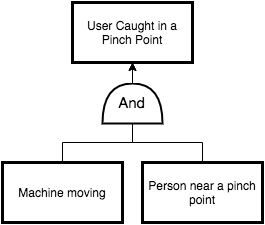
\includegraphics[width=0.35\textwidth]{PinchPointFTA.png}
\captionof{figure}{FTA for a user caught in a pinch point.}
\label{fig:yRailFig}
\end{center}

\newpage
\subsection{Harmful Pneumatic Activation}
\textbf{Description}\\
The pneumatic actuator will involve a very fast-moving component in order to strike the cue ball with sufficient force. If there is something in the way of the end-effector other than the cue ball such as the table, other parts of the machine, or a person, there is likely to be resulting damage.\\~\\
\textbf{Plans for Avoidance/Mitigation}\\
When the machine is about to take a shot a warning message or sound can be audibly played by the controller in order to alert the user to the upcoming movement. The machine will pause after this sound to allow the user time to stop the machine if there is an issue.\\~\\
The following diagram provides specific details for this hazard:\\
\begin{center}
	\includegraphics[width=0.35\textwidth]{PneumaticFTA.png}
\captionof{figure}{FTA for harmful pneumatic activation.}
\label{fig:yRailFig}
\end{center}

\newpage
\subsection{Jumping Pool Balls}
\textbf{Description}\\
Pool balls have a tendency to jump off the table if struck in a certain way. If the ball bounces off of the table, there is potential for damage to the machine, the surrounding environment, or a person.\\~\\
\textbf{Plans for Avoidance/Mitigation}\\
The end-effector will be designed in such a way that even when striking at its maximum force, the pool balls will never lose contact with the table. However, the user will still be playing on the table and might jump the balls. There is not much able to be done in terms of protecting other people or the surrounding environment unfortunately but the machine itself will be made in such a way that it is durable in areas where a jumping ball will be likely to hit it.\\~\\
The following diagram provides specific details for this hazard:
\begin{center}
	\includegraphics[width=0.9\textwidth]{JumpingBallsFTA.png}
\captionof{figure}{FTA for jumping pool balls.}
\label{fig:yRailFig}
\end{center}

\newpage
\subsection{Dangerous Machine Traversal}
\textbf{Description}\\
While the machine is traversing, anything in the way may be at risk. For example, depending on the speed, there could be damage due to impact. Another less severe example could involve knocking off items on the edges of the table.\\~\\
\textbf{Plans for Avoidance/Mitigation}\\
In order to avoid high speed impacts, the controller will simply not permit motion faster than a certain, safe speed. In terms of the knocking of items off the table, a warning will be printed in a visible location on the system in order to warn users of that risk. In addition, a warning message or sound can be audibly played by the controller in order to alert the user to upcoming movement. The machine will pause after this sound to allow the user time to stop the machine if there is an issue.\\~\\
The following diagram provides specific details for this hazard:
\begin{center}
	\includegraphics[width=0.9\textwidth]{DangerousTraversalFTA.png}
\captionof{figure}{FTA for dangerous machine traversal.}
\label{fig:yRailFig}
\end{center}

\newpage
\subsection{Loose Objects Snagged}
\textbf{Description}\\
At various locations -- namely the pinch points listed earlier as well as the rotational motor on the end-effector base and the belts on the x- and y-rails -- loose clothing, jewellery or long hair may be caught and pulled in. If these objects are attached to a person, this can lead to strangulation or being pulled into dangerous areas of the machine.\\~\\
\textbf{Plans for Avoidance/Mitigation}\\
For this hazard protective guards will be mounted around moving parts in order to prevent the machine from snagging loose objects. Additionally, emergency stop buttons will be located within reach of all moving parts in the case that an object should become snagged. Lastly, a warning will be printed in a visible location on the system in order to warn users of this risk.\\~\\
The following diagram provides specific details for this hazard:
\begin{center}
	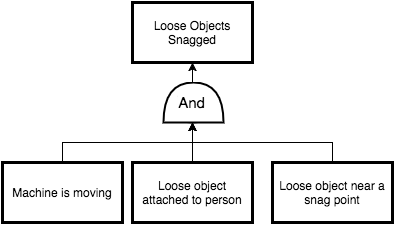
\includegraphics[width=0.5\textwidth]{LooseObjectFTA.png}
\captionof{figure}{FTA for loose objects being snagged.}
\label{fig:yRailFig}
\end{center}

\newpage
\subsection{Sensor Interference by Outside Sources}
\textbf{Description}\\
The machine makes use of delicate sensors in order to facilitate safe and accurate motion along the x-rail, y-rail, and rotation arm. Should these sensors be interfered with such that they no longer generate expected results the performance of the machine will be jeopardized. Physical activation of the sensors by outside sources can cause the machine to lose track of it's current position thus resulting in faulty shot taking. Deactivation of the sensors can cause the machine to run into the ends of the x and y rails, thus resulting in damage to the machine.\\~\\
\textbf{Plans for Avoidance/Mitigation}\\
In order to avoid physical interference to the sensors by outside sources the sensors will be encased in protective shielding that will make it difficult for accidental manual activation to occur. Furthermore, the sensors will only be monitored by the software system while the machine is in motion. Any physical interference which occurs during the user's turn (user operation) will thereby be ignored. In order to avoid undesired deactivation of sensors the sensor wiring will be encased in durable heat shrink tubing and will be closely affixed to the machine so as to minimize potential catch points.\\~\\
The following diagram provides specific details for this hazard:
\begin{center}
	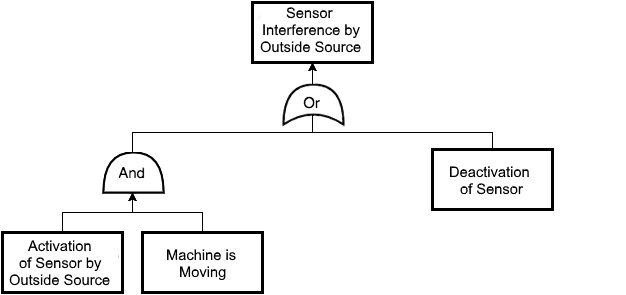
\includegraphics[width=0.8\textwidth]{SensorInterferencerFTA.png}
\captionof{figure}{FTA for sensor interference by outside sources.}
\label{fig:yRailFig}
\end{center}

\newpage
\subsection{Non-Responsive UI}
\textbf{Description}\\
The machine makes use of user input buttons in order to allow the user to control the machine. The functionality of the user buttons allows the user to inform the machine that: the user wishes to take a turn (stop all automated machine functionality), the user wishes for the machine to take a turn, or the user wishes for the machine to move/stop moving to either ends of the table such that the user can take an unobstructed shot. In the case that these user controls should become unresponsive the performance of the machine can become undesirable and therefore dangerous.\\~\\
\textbf{Plans for Avoidance/Mitigation}\\
In order to mitigate the likelihood of unresponsive UI the system will be designed such that reliablility of user buttons are a priority. The action of a button press should give reliable and repeatable results. The system will be thoroughly tested to ensure that the hardware and software associated with user buttons are robust and responsive. Furthermore, in the event that UI becomes unresponsive there will be an emergency shut off switch located near the user buttons which when thrown will introduce a break in the power supply of the circuit and stop all motion of the machine.\\~\\
The following diagram provides specific details for this hazard:
\begin{center}
	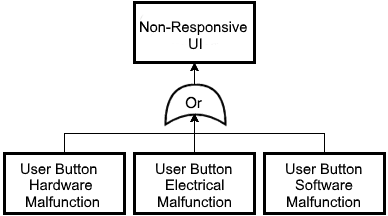
\includegraphics[width=0.5\textwidth]{NonResponsiveUIFTA.png}
\captionof{figure}{FTA for non-responsive UI.}
\label{fig:yRailFig}
\end{center}

\newpage
\subsection{Overheating}
\textbf{Description}\\
The machine makes use of high-torque stepper motors to facilitate motion in the x, y and r directions. These motors draw high levels of current and are controlled through the use of motor controllers hooked into the $\mu$C. The motor controllers can generate a considerable level of heat during normal operation of the machine. This heat may result in injury to any users who come in contact with the motor controllers or may result in destruction of the motor controllers themselves.\\~\\
\textbf{Plans for Avoidance/Mitigation}\\
In order to mitigate the threat of injury from user interaction with high temperature components the $\mu$C with attached motor controllers will be isolated via ventilated and thermally resistant protective shielding. Furthermore, each motor controller will have a heatsink attached via thermally conductive adhesive. This will serve to protect the controllers from destruction due to overheating.\\~\\
The following diagram provides specific details for this hazard:
\begin{center}
	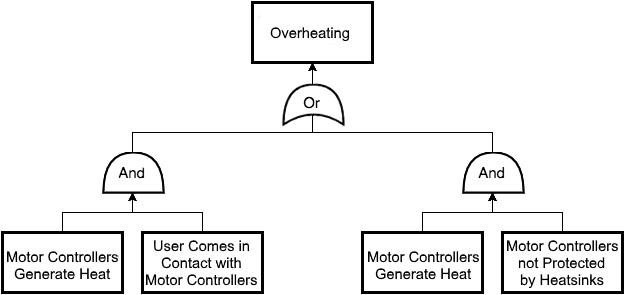
\includegraphics[width=0.8\textwidth]{OverheatingFTA.png}
\captionof{figure}{FTA for overheating.}
\label{fig:yRailFig}
\end{center}

\newpage
\subsection{Electric Shock}
\textbf{Description}\\
The machine has motor leads running along the sides of the pool table, wires connecting the sensors distributed along the table to the $\mu$C, and wires to connect the $\mu$C to power. Some of these wires are prone to tear since they will be extended and twisted as the system traverses over the table. The wires may also be accidentally pulled by the user and break as a result. If the insulation on any of these wires is broken it could pose as an electric shock hazard to a user operating the system.\\~\\
\textbf{Plans for Avoidance/Mitigation}\\
In order to mitigate the threat of injury from electric shock all wires will be neatly tucked into the system as to not interfere with a user operating the system. Wires will be affixed so as to keep wire slack from hanging, this will act to mitigate a tripping hazard in addition to electric shock.\\~\\
The following diagram provides specific details for this hazard:
\begin{center}
	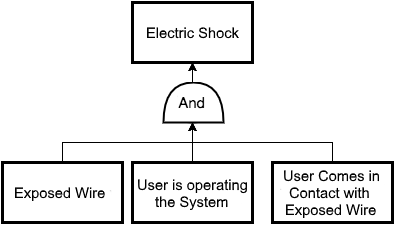
\includegraphics[width=0.5\textwidth]{ElectricShockFTA.png}
\captionof{figure}{FTA for Electric Shock.}
\label{fig:yRailFig}
\end{center}

\newpage
\subsection{Motion Interference}
\textbf{Description}\\
Since the user will be playing very closely to the machine there is high potential for outside interference to the system's motion. The timing belt is a primary source of interference since it is sensitive to wear. If the timing belt wears out it may potentially slip, causing unintentional movement of the system. Motors are another source of interference. If a set of motor leads should become disconnected while the system is in operation the machine's ability to traverse above the table will be restricted. Lastly, if a foreign object gets in the way of the machine while it is in motion this would result in interference to the system. \\~\\
\textbf{Plans for Avoidance/Mitigation}\\
In order to mitigate any unintentional sources of interference the system will only begin its turn once the user presses a button. The system will also use a colour-changing LED light to indicate that it will begin moving. This will inform the user to step back from the machine. The system will be programmed to only trigger the endstop interrupts when the machine is in motion, so if the user activates the endstops during their turn the system will be unaffected. The motor leads will be tucked away neatly and out of the way so as to prevent accidental snagging of the wires. \\~\\
The following diagram provides specific details for this hazard:
\begin{center}
	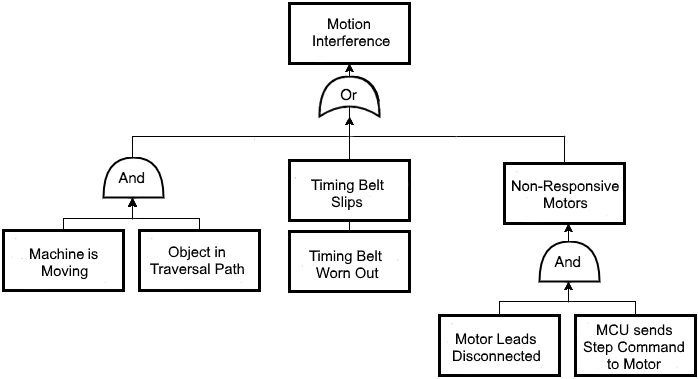
\includegraphics[width=0.9\textwidth]{MotionInterferenceFTA.png}
\captionof{figure}{FTA for Motion Interference.}
\label{fig:yRailFig}
\end{center}

\end{document}


